\section{Udvikling af programmet}
	\begin{frame}{Udvikling af programmet}\framesubtitle{Indhold}
		 \begin{itemize}
		 	\item Arkitektur
		 	\item Funktionskomponenter
		 	\item Modellag
		 	\item Programmering
		 	\item Teknologier
		 	\item API
		 \end{itemize}
	\end{frame}
	\subsection{Arkitektur}
		\begin{frame}[t]{Arkitektur}\framesubtitle{MVC \& Komponenter}
			\begin{columns}[T]
				\begin{column}{.48\textwidth}
					\begin{itemize}
						\item Website
						\item Client--Server arkitektur
						\item MVC
						\begin{itemize}
							\item Model
							\item View
							\item Controller
						\end{itemize}
						\item Opdelt i funktionskomponenter
					\end{itemize}

				\end{column}
				\begin{column}{.48\textwidth}
					\begin{figure}
						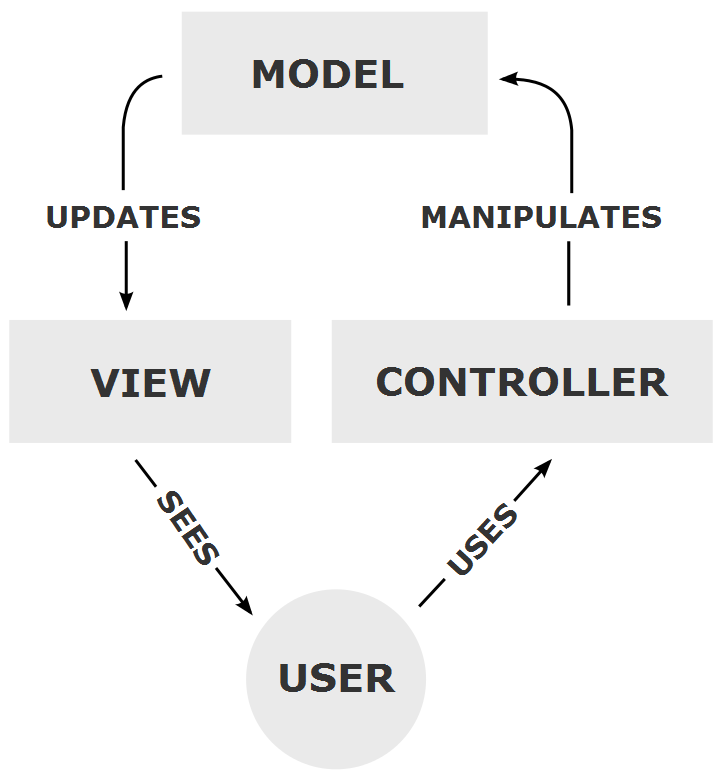
\includegraphics[width=1\textwidth]{images/MVC_2.png}
						\caption{MVC, figur af RegisFrey fra \url{wikipedia.org}}
					\end{figure}
				\end{column}
			\end{columns}
		\end{frame}
		
		\subsubsection{Funktionskomponenter}
		\begin{frame}[t]{Arkitektur}\framesubtitle{Funktionskomponenter}
			\begin{itemize}
				\item Funktionskomponenters adgange og afhængighedder
				\item Rækkefølge af komponenters implementering
			\end{itemize}
			%Topologisk sortering -> omvend reækkefølge -> implementer
			%Bruger > Tilbud > Indkøbsliste > Overvågning > Opskrift
			\vspace{-5pt}
			\begin{figure}[h!]
				\centering
				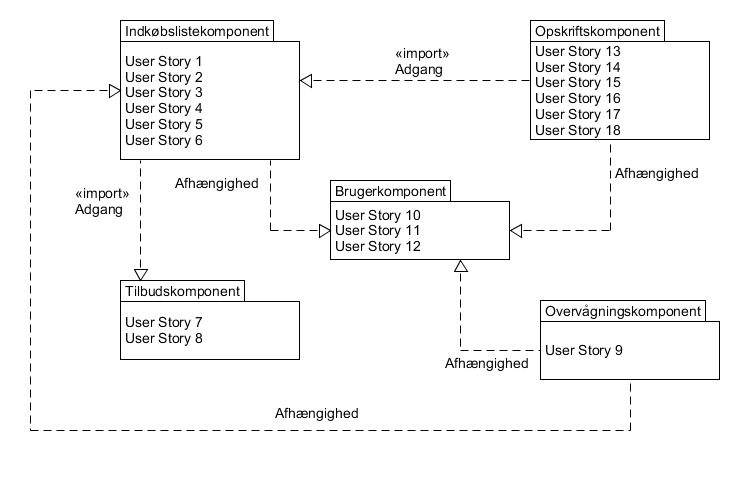
\includegraphics[width=1\textwidth]{images/Komponenter.png} % trim=1.4cm 6.1cm 6.5cm 1.8cm, clip, 
			\end{figure}
		\end{frame}

		\subsubsection{Modellag}
			\begin{frame}[t]{Arkitektur}\framesubtitle{Modellag}
				\begin{figure}
					
					\includegraphics<1-2>[trim=8.2cm 16.5cm 0.5cm 6.3cm, clip, width=1\textwidth]{images/PF_Model_UML_Simple.pdf} % ttrim=1.4cm 6.1cm 6.5cm 1.8cm, clip,
					\includegraphics<3>[width=0.5\textwidth]{images/UML_Pref_med_felter.png} % ttrim=1.4cm 6.1cm 6.5cm 1.8cm, clip,

				\end{figure}
				\begin{itemize}
					\item<2> Many-To-Many via bindeklasser med attributter
					\item<3> Problemer med modellaget
				\end{itemize}
			\end{frame}
		
		\subsection{Programmering}
			\begin{frame}{Programering}
				\begin{columns}
					\begin{column}{.48\textwidth}
						\begin{itemize}
							\item Git
							\begin{itemize}
								\item Branching
								\item Code-review
							\end{itemize}
							\item Pair Programming
							
						\end{itemize}

					\end{column}
					\begin{column}{.48\textwidth}
						\textbf{Branches:}
						\begin{itemize}
							\item master
							\item develop
							\item feature-xyz
							\item bugfix-abc
						\end{itemize}
					\end{column}
				\end{columns}
			\end{frame}


		\subsection{Teknologier}
			\begin{frame}[t]{Teknologier} %\framesubtitle{Udvikling intro}
				\begin{itemize}
					\item<1> ASP.NET
					\begin{itemize}
						\item<1> MVC
						\item<1> Razor view engine
						\item<1> Login system
					\end{itemize}
					\item<2> Entity Framework
					\begin{itemize}
						\item<2> Object--relational mapping
						\item<2> Code--first
						\item<2> Migrations
					\end{itemize}
					\item<3> Bootstrap
					\begin{itemize}
						\item<3> Responsiv layout
						\item<3> CSS--klasser og JS
					\end{itemize}
				\end{itemize}
			\end{frame}

		\subsection{eTilbudsavis API}
			\begin{frame}[t]{eTilbudsavis API}
			Kommunikation med API'en:
				\begin{enumerate}
					\item<1> POST api.etilbudsavis.dk/v2/\textbf{sessions}?api\_key=[...]
					\begin{itemize}
						\item<1> Modtag \texttt{token}
						\item<1> Beregn \texttt{signature} (SHA-256)
					\end{itemize}
					\item<2> GET api.etilbudsavis.dk/v2/\textbf{offers}?r\_lat=57\&r\_lng=9
					\begin{itemize}
						\item<2> Modtager 100 tilbud som JSON
						\item<2> Gentages til alle er modtaget (do..while)
						\item<2> Konverteres til \texttt{Offer}--klassen
					\end{itemize}
				\end{enumerate}
				\begin{itemize}
					\item<3> Er tidskrævende (60-300 sekunder)
					\item<3> Kan muligvis paralelliseres for bedre hastighed
					\item<3> Dataet kunne være bedre
				\end{itemize}
			\end{frame}